\documentclass[
  a4paper,
  % twoside
]{report}

\title{Immutable package management for Linux}
\author{Fernando Ayats Llamas}

% Better fonts
\usepackage{fontspec}
\setmainfont{texgyrepagella}[
  Extension = .otf,
  UprightFont = *-regular,
  BoldFont = *-bold,
  ItalicFont = *-italic,
  BoldItalicFont = *-bolditalic,
  ]
\setmonofont{iosevka-normal-medium.ttf}[
  SizeFeatures={Size=10},
  Contextuals={Alternate},
  NFSSFamily={iosevka-normal}
]

% Bibliography (no bibtex)
\usepackage[backend=biber]{biblatex}
\addbibresource{assets/miq.bib}

\usepackage{graphicx}
\usepackage{svg}
\svgsetup{inkscapelatex=false}


\usepackage{xurl}


\usepackage[colorlinks]{hyperref}
\usepackage{xcolor}
% \hypersetup{pdfborder = {0 0 0}} % no boxes around links
\definecolor{MK_One_One}{RGB}{140,81,10}
\definecolor{MK_One_Two}{RGB}{216,179,101}
\definecolor{MK_One_Three}{RGB}{246,232,195}
\definecolor{MK_One_Four}{RGB}{199,234,229}
\definecolor{MK_One_Five}{RGB}{90,180,172}
\definecolor{MK_One_Six}{RGB}{1,102,94}
\hypersetup{
 linkcolor=MK_One_One
,citecolor=MK_One_Two
,filecolor=MK_One_Three
,urlcolor= MK_One_Six
,menucolor=MK_One_Five
,runcolor=MK_One_Four
,linkbordercolor=MK_One_One
,citebordercolor=MK_One_Two
,filebordercolor=MK_One_Three
,urlbordercolor=MK_One_Six
,menubordercolor=MK_One_Five
,runbordercolor=MK_One_Four
}


\usepackage{lipsum}

\usepackage{acronym}

\usepackage{listings}
\lstMakeShortInline[columns=fixed]|
\lstset{
  basicstyle=\ttfamily,
  basewidth=0.5em
}

% custom headings
% \usepackage{fancyhdr}
% \pagestyle{fancy}
% \fancyhf{}
% % \lhead{\rightmark}
% % \rhead{Página \thepage}
% %% \cfoot{\today}
% \fancyhead[LE,RO]{\rightmark}
% \fancyhead[RE,LO]{Page \thepage}
% \fancyfoot[CE,CO]{Fernando Ayats Llamas - \today}

\usepackage[outputdir=aux]{minted}

% https://tex.stackexchange.com/questions/16582/center-figure-that-is-wider-than-textwidth
\makeatletter
\newcommand*{\centerfloat}{%
  \parindent \z@
  \leftskip \z@ \@plus 1fil \@minus \textwidth
  \rightskip\leftskip
  \parfillskip \z@skip}
\makeatother

\usepackage{placeins}

\usepackage{tabularray}

\begin{document}


\begin{abstract}
  \lipsum[3]

\end{abstract}
\newpage

% \renewcommand{\abstractname}{Acknowledgements}
% \begin{abstract}
%   \lipsum[3]

% \end{abstract}
% \newpage


\begin{titlepage}
  \tableofcontents
\end{titlepage}




\chapter{Introduction}


To understand the problems of the classical software deployment model, we need
to take a step back into its origins. We can go back to the seventies, when the
Unix system was born. The design of file system became the basic design
component of Unix  \cite{ritchieUNIXSystemEvolution1984} . The idea was to be able to interface
with all the devices available to the operating system, as if they were regular
files. For this reason, the layout of this file system was of great importance.
Every file (which include device nodes) is placed as a child of the root
directory |/| . Then, the first level of directories organizes the overall
structure of the system. As Linux distributions emerged and developed, this
structure was preserved, and became the \ac{FHS}
\cite{FHSLinuxFoundation}.

In the \ac{FHS} deployment model, files are organized by separate packages, and the
collected into common directories, such as |/bin| for executable files, or
|/include| for header files. This model provides some advantages, such as

\begin{itemize}
    \item Common place for every file type, which makes it easier to
        find them.
    \item Packages share their common dependencies, which reduces the
        amount of disk space used.
\end{itemize}

To share a dependency, a package |A| only has to use the absolute path to the
file from package |B|, which is known. For example, if package |A| has a binary
|/bin/A| which depends on the library |B| at |/lib/libB.so|, and |C| also
depends on it, we can draw the dependency graph on figure \ref{fig:graph1}.

\begin{figure}
    \centering
    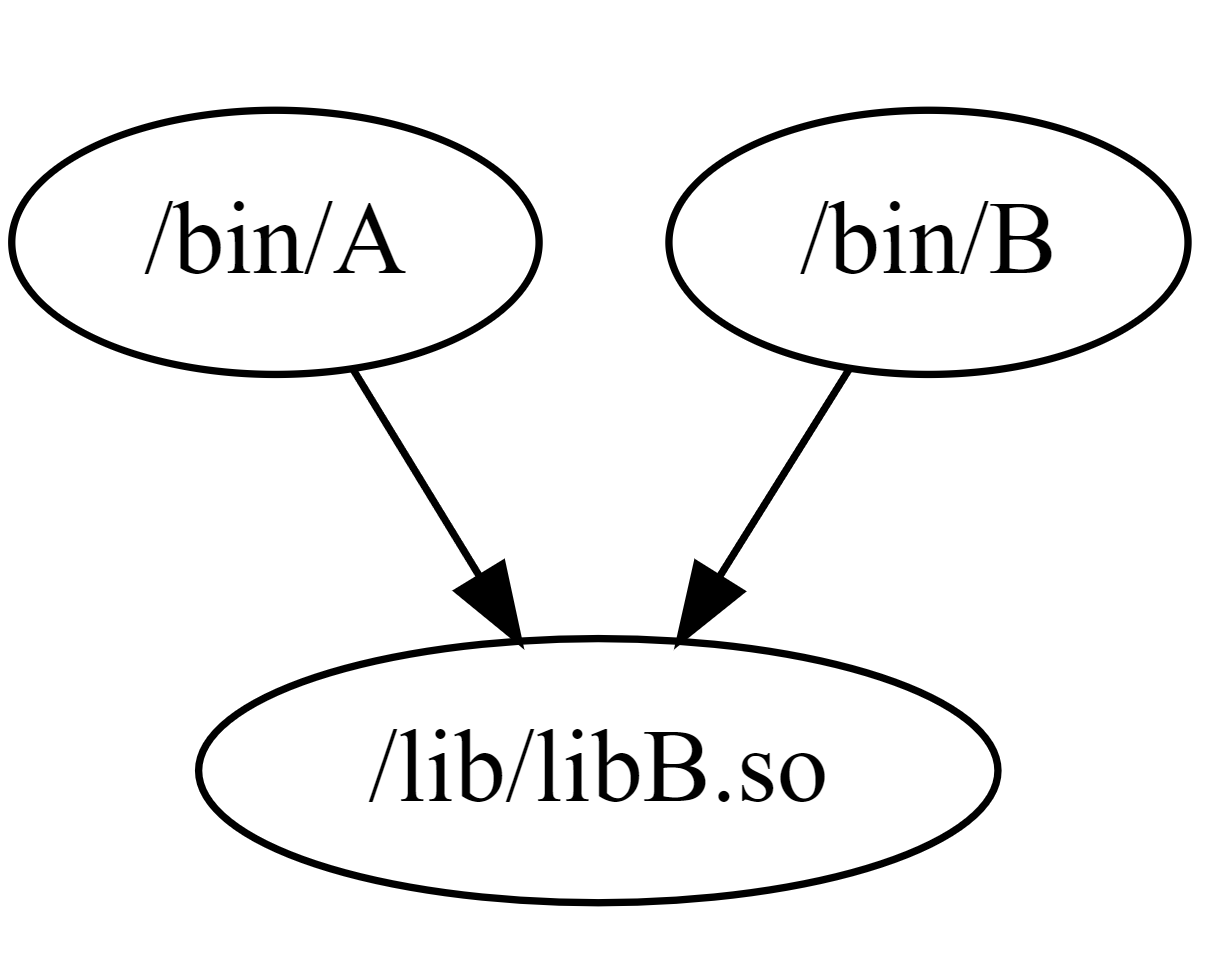
\includegraphics[width=0.3\textwidth]{Screenshot 2023-05-29 150312.png}
    \caption{Dependency graph of packages A, B and C.}
    \label{fig:graph1}
\end{figure}

This model then couples the dependency graph of the packages, with the structure
of the file system. This means, that not every dependency graph is possible to
be constructed on disk, because we must follow the rules of the file system. For
example, if package |A| wants to use the path |/bin/A|, and package |A'| wants
to use it too, this dependency graph is not possible to be constructed, as we
have a conflict. This is illustrated on figure \ref{fig:graph2}.

\begin{figure}
    \centering
    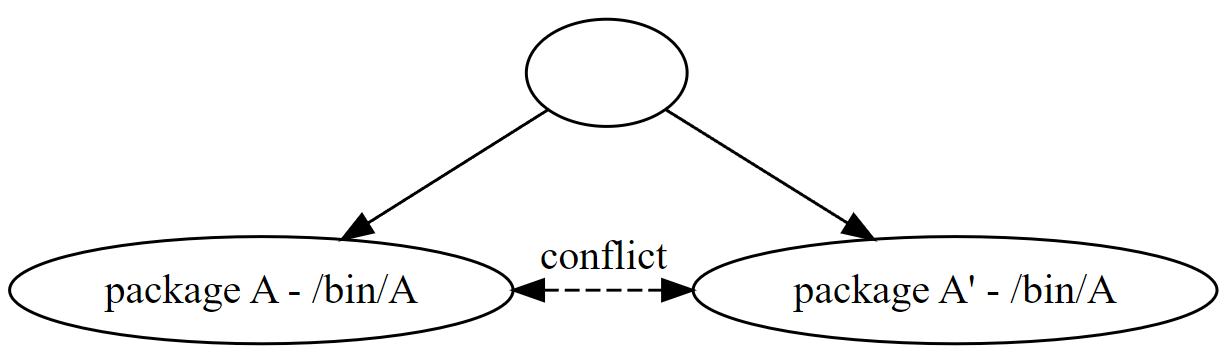
\includegraphics[width=0.4\textwidth]{Screenshot 2023-05-29 153351.png}
    \caption{Dependency conflict of packages A and A' .}
    \label{fig:graph2}
\end{figure}

A more subtle problem is the Circular Dependency Problem \cite{al-mutawaShapeCircularDependencies2014}. This problem stems
from using an imperative way of managing the dependencies, that is, the usage of
a \ac{CLI} to install or remove packages one after the
other. After requesting some operation on the dependency graph, the result could have
loops in it, as illustrated on figure \ref{fig:graph3}. This causes problems in
the ordering of the operations, and many others. Coloquially, this is known refered to as
``dependency hell'' \cite{abateDependencySolvingStill2020}, denoting the difficulty of managing the dependencies of a system.

\begin{figure}
    \centering
    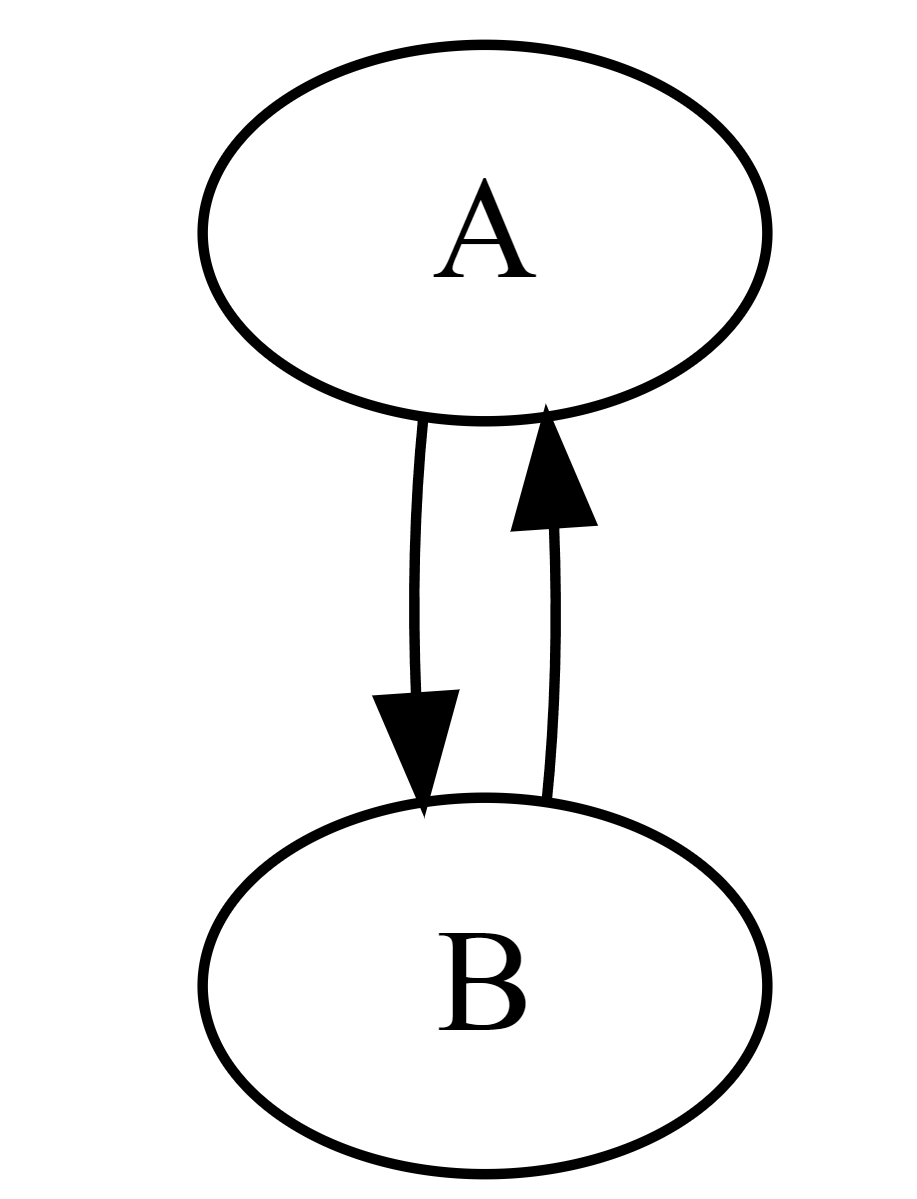
\includegraphics[width=0.2\textwidth]{Screenshot 2023-05-29 154056.png}
    \caption{Circular dependency between A and B.}
    \label{fig:graph3}
\end{figure}

What it is proposed then, is a system where the dependency graph is decoupled
from the file system. This means, that packages don't rely on standard locations
to look for files. Therefore, the \ac{FHS} is not used anymore --- or at least, not
in the same way. The previous work of the Linux distributions
NixOS \cite{dolstraPurelyFunctionalSoftware2006} and Guix System
\cite{courtesFunctionalPackageManagement2013} or Spack, the \ac{HPC} package
manager \cite{gamblinSpackPackageManager2015}, already paved the way into this idea.

In miq (pronounced [miku]), the packages are evaluated into a \ac{DAG}, in which
each node represents a package, and each edge represents a dependency. Then,
each node gets a unique identifier, which depends on its own definition, and the
identifier of its dependencies. This ``identifier'' is represented as a
cryptographic hash. Finally, each package receives a directory in the filesystem
unique to its identifier, as shown on figure \ref{fig:graph4}.


\begin{figure}
    \centering
    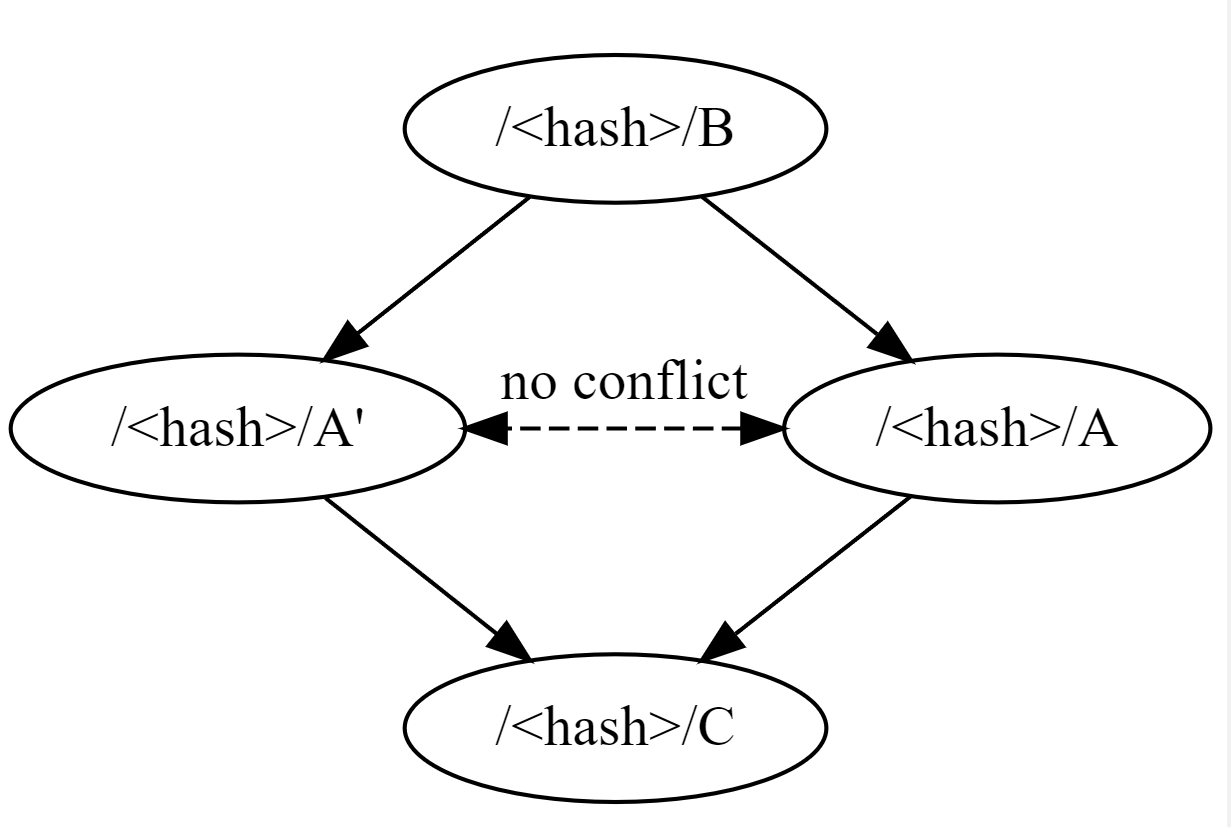
\includegraphics[width=0.4\textwidth]{Screenshot 2023-05-29 164148.png}
    \caption{Dependency graph of packages A, A', B and C, by using a unique prefix.}
    \label{fig:graph4}
\end{figure}



This system also provides a way to transverse the dependency graph, and look for
any change in the transitive dependency graph. For example, if package |A|
depends on |C| through |B|, a change on |C| triggers a change of its hash. Which
in turns, triggers a change on |B|, and then on |A|. With this system, the full
dependency graph is known. A common problem in Linux is "my application works on
my machine" \cite{mukherjeeFixingDependencyErrors2021}. Even even the application itself is the same, we still rely on
files provided from the system via the \ac{FHS} and the package manager.

Finally, this enables a deployment model where updates don't require modifying
files in place. Traditionally, if we want to update a package with files
|/bin/A| and |/bin/B|, these files are modified in place. This means, that if
there is any problem during the transaction (like a power outage or a disk
failure), the system is left in an inconsistent state. In miq, the original
package would still be available on its old path, and we can delay the update to
just swapping a symlink into the current version.

The main solution to this problem currently is the usage of containers. A
container is a collection of files, which can be thought as Linux distribution
itself \cite{DockerAcceleratedContainerized2022} \cite{merkelDockerLightweightLinux2014}. This container is then run by a ``runtime'', that isolates it from the
host's filesystem, as shown in figure \ref{fig:graph5} . As a result, the files in the container don't conflict with
the hosts, or other containers. The main way to deploy applications is then
using one container per application, which bundles its entire dependency tree.
Because the underlying filesystem of each container has the same problems as any
other, the containers solution moves the problem into a singular image, which
contains a single application, and as a result a smaller dependency footprint.

In contrast to miq, where each dependency lives in its own directory, without
collisions and need for a sandboxing runtime, as illustrated in figure
\ref{fig:graph6} .

\begin{figure}[hbt]
    \centering
    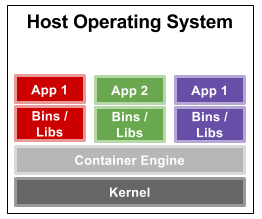
\includegraphics[width=0.4\textwidth]{Screenshot 2023-05-29 173501.png}
    \caption{Deployment model of containerized applications.}
    \label{fig:graph5}
\end{figure}

\begin{figure}[hbt]
    \centering
    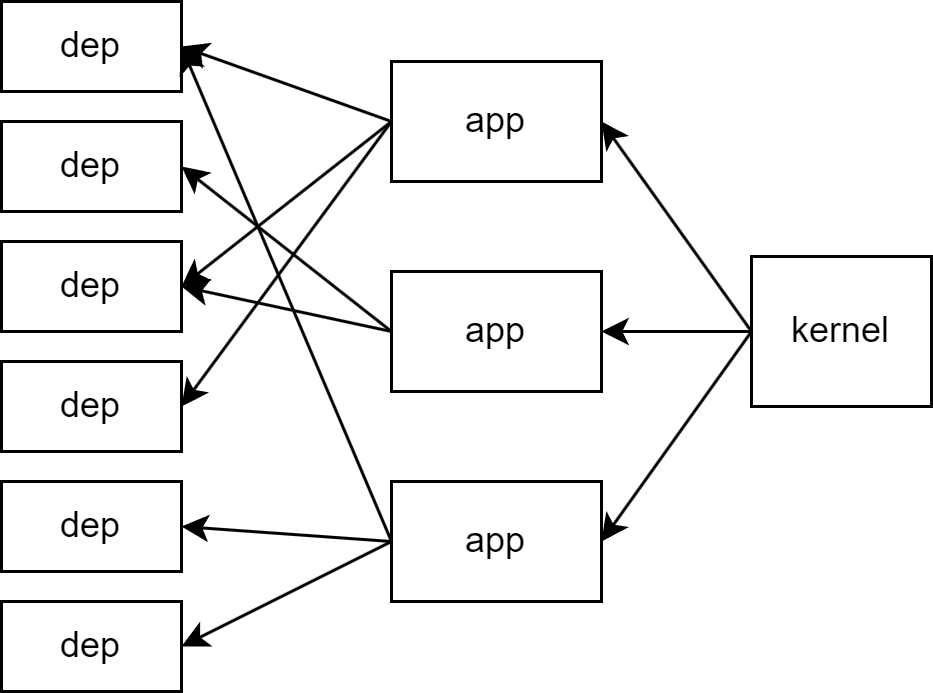
\includegraphics[width=0.4\textwidth]{dep2.png}
    \caption{Deployment model of miq.}
    \label{fig:graph6}
\end{figure}




\chapter{State of the art}

The landscape of Linux is separated by what is called as
``Linux distribution''. A Linux distribution (or distro for
short) is a collection of packages that are distributed
together as a part of the project. A package is a software
project that is distributed as a single unit, and contains
multiple files in the disk. The packages vary from the most
basic libraries and programs, like libc or bash, to any
complex software, like Google Chrome -- and also the Linux
kernel itself along with its kernel modules.

Linux packages are not meant to be shared between different
distribution. When a package is distributed for a specific
distro -- for example, Ubuntu -- it relies on libraries
provided by other Ubuntu packages. If we try to install this
package into a different distribution, for example Fedora,
it may or may not work. This problem is aggravated by the
fact that Linux libraries are very ``split'', as following
the UNIX philosophy of ``do one thing and do it well'', the
state of Linux distributions is that there are many
libraries that combine. The vast majority of these library
are written in C and C++, making Linux package managers the
de facto package manager for these languages
\cite{amor-iglesiasMeasuringLibreSoftware2005} . This is in
contrast to
other operating systems like Windows, where a package author
can rely on a ``base'' system that doesn't change, and can
bundle its own dependencies as part of the package, without
intermediate links.

Because each distribution has its own organization of
packages versions and customization, that are not
interoperable between different distributions, the Linux
ecosystem is very fragmented
\cite{espePerformanceEvaluationContainer2020}, even existing
distributions for specific applications
\cite{nemotoLin4NeuroCustomizedLinux2011} . The projects
use their own
package manager to install every package, as installing a
different package manager is not guaranteed to work. For
this reason, each distribution is only associated with its
reference package manager, being two sides of the same coin.
Some examples are:

\begin{itemize}
    \item Debian --- apt
    \item Fedora --- dnf
    \item Gentoo --- portage
    \item Arch --- pacman
\end{itemize}

With the increasing usage of internet services, Linux has
placed itself as the de facto operating system for servers.
As the online infrastructure of the world runs on Linux,
there is an increasing amount of developers that need to
deploy their applications into cloud services. One problem
that developers face is that applications are not portable
enough between different Linux distributions. This is partly
a result of this fragmentation that was mentioned earlier.
Updates of the same distribution can also cause
incompatibilities from one version to another.

As a result, an alternative software deployment solution to
just building and running packages in the host operating
system was developed by the company \textit{Docker}, and
later established in 2015 under the Linux Foundation as the
\textit{Open Container Initiative}. This solution uses the
concept of ``containers'', which are a collection of files
that run in a sandboxed environment from the host operating
system. This environment is usually based on some Linux
distribution such as Debian, but with the advantage that a
container may be built from any host \ac{OS} and deployed
into any host \ac{OS} .

Containers serve as a ``compatibility layer'' for classical
Linux distributions, as it doesn't change the underlying
functionality of packages themselves. But it is effective
enough to provide a good developer experience.

Earlier on the timeline, \citeauthor{dolstraNixOS2008}
researched this same problem of the classical software
deployment, and proposed a solution based on the concept of
a functional package manager \cite{dolstraNixOS2008} . After
years of development, this project has evolved into the Nix
package manager and the NixOS Linux distribution. Nix tries
an alternative approach to the classical package managers,
by prefixing each package with a unique path based on a hash
of its definition and dependencies. This allows multiple
packages to coexist in the same host operating system, and
also to use Nix on different host systems that are not
NixOS. While this solves the problem of reproducible
software deployments that Docker / OCI solves, the latter
also provides an application runtime which is used to
isolate the application from the host operating system \cite{espePerformanceEvaluationContainer2020}. In
this regard, Nix is just a system to build packages. One of
the problem that Nix faces is the usage of its own
language Nix (with the same name), that is based on the
concept of functional programming and pure function
application, with the inspiration of Haskell. As this
language is not very user-friendly, the GNU Guix project
investigated in the usage of the Scheme language as an
alternative to Nix
\cite{courtesFunctionalPackageManagement2013} .

A different approach to the problem of mutating packages in
the operating system has been taken by OSTree. This project
aims to develop a package-centric installation model based
on git \cite{waltersFutureContinuousIntegration2013} . In
the OSTree-backed distributions, like Fedora Silverblue, the
operating system is stored in a ostree, such that changes
updates are done by pulling a new ``commit'' from the
internet. This change is done automatically without user
intervention, such that the files in the operating system
are not swapped while the system is online. As ostree
organizes the file in a git-like structure, the \ac{FHS} is
kept (|/usr/bin|, |/usr/lib|, etc.), but the files are stored
in a content address storage. The file system is also kept
as read-only, as the changes are performed on boot, thus
having an immutable system.

While package managers for Linux operating systems are on
the spotlight of this project, any software project grows
big enough such that it needs to implement its own package
manager. This is the case for every programming language,
that supports any kind of concept of libraries, such as the
languages used for this project: Rust (crates) and Lua
(luarocks). The reproducibility of packages is of serious
concern \cite{goswamiInvestigatingReproducibilityNPM2020}, as the world relies more heavily on online
services.


\chapter{Overview}

The result of this research was the development of |miq|, a package manager and
build system for Linux.

Miq is a single-file executable that handles the full lifecycle of the build
process of the packages it manages. These stages include:

\begin{enumerate}
    \item Evaluating the expressions that describe packages
    \item Calculating the dependency graph
    \item Fetching the necessary source code
    \item Performing the described build process
    \item Handling the storage and tracking of the installed packages
\end{enumerate}

Therefore, the following sections will all the components that make up miq, and
their interactions.

\section{Unique identifiers}

The development of miq aimed for a modular design, such that
each component didn't have much coupling with the others.
This allows for easy refactoring of parts of the source
code, while leaving the rest of the system untouched. As
such the components of miq can be laid out in figure
\ref{fig:miq-components} .

\begin{figure}[hbtp]
    \centerfloat
    % 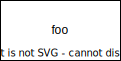
\includegraphics{assets/overview.png}
    \includesvg[width = 450pt]{assets/overview.svg}
    \caption{Overview of the subsystems of miq}
    \label{fig:miq-components}
\end{figure}

Miq is presented as a pipeline of stages, where each
subsystem transforms the input data to achieve a desired
state. This design is inspired by other package managers,
which present a similar structure of stages. The main
difference, is that miq works on static package laid out in a file, which describe the desired state of the
system. In contrast to other package managers, like |apt|,
where the final state of the system is a succession of
commands executed in the shell.

On of the main differences of miq to other package managers,
is how the files are laid out in the file system. This is
because each package is given a unique identifier, which in
turns is used for the directory where the package will be
located. This identifier is also unique between different
versions of the same package. And not only that, but it also
encodes the recipe used to build the package itself, and all
of its parents.

To accomplish the tagging of each package with a unique
identifier, a flow of data from package input to package is
visualized on figure \ref{fig:hash}. From a |PackageInput|,
a unique hash is generated, that is the result from hashing
all the fields of the struct. Finally, the hash (an unsigned
32-bit integer) is encoded into text, to form the name of
the package. For this application, the algorithm used is the
\textit{Fowler-Noll-Vo} hash function, which is implemented
in the |fnv| create \cite{FnvRust} . This hash function is
not cryptographically secure, but this was not one of the
design requirements of miq (and can be swapped out for any
other hashing algorithm as needed, as long as it conforms to
the |Hash| trait in Rust).



\begin{minted}{rust}
#[derive(Hash)]
struct PackageInput {
    name: String,
    version: Option<String>,
    script: MetaTextInput,
    deps: Option<Vec<Unit>>,
    env: Option<BTreeMap<String, MetaTextInput>>,
}
\end{minted}

\begin{figure}[hbtp]
    \centerfloat
    \includesvg[width = 0.7\paperwidth ]{assets/hash.svg}
    \caption{Overview of the hashing algorithm}
    \label{fig:hash}
\end{figure}

The implications of this design is that any package gets a
different place on the file system, which is derived from
everything that defines the package itself - its build
script and its dependencies, which in turn are also hashed
by the same rules. The advantage of this design, is that
every package has its dependencies perfectly defined,
instead of relying on automatic detection. Let's say that
package |foo| depends on package |bar|. On a conventional
package manager, if |bar| is changed in any form (for
example, updated), then |foo| is usually not modified. But
in essence, now |foo|, if we consider it as a whole, that is
its whole dependency tree, it has changed. This poses a big
issue for the reproducibility of an operating system. Is
|foo| the same if we swapped |bar| for a different version?
Or if we swapped one of |bar|'s dependencies? (Figure
\ref{fig:depswap}) In miq, it is clear that the packages are
no longer the same, as the hashes of its entire dependency
tree has changed, and therefore the name of the output
package. This means that a package "foo" does not really
exist in miq, but rather a package "foo" with a specific hash.

\begin{figure}[hbtp]
    \centerfloat
    \includesvg[width = 200pt]{assets/depswap.svg}
    \caption{Change of dependencies for a package for a conventional package manager}
    \label{fig:depswap}
\end{figure}

% insert depswap-miq.svg
\begin{figure}[hbtp]
    \centerfloat
    \includesvg[width = 200pt]{assets/depswap_miq.svg}
    \caption{Change of dependencies for a package for miq}
    \label{fig:depswap_miq}
\end{figure}

\FloatBarrier
\section{Graph-based dependency resolution}

In software deployment, one of the main goals is to have be
able to reproduce a deployment environment as reliably as
possible. This means that any external factors should be
reduced to a minimum, such that the end result is as close
to the expected as possible. The reality of system
deployments is that not all environments are the same, such
that the same deployment can be applied to different systems
with different hardware -- for example, different network
cards, hard drives or even different architectures.

On the software side, the same problem exists. Any
deployment is composed of different parts of software which
interact with each other. To reduce any external factors,
a possible solution is to try to control the entire software
stack -- from the kernel, to the operating system and
libraries and finally to the application to be deployed.
This can be seen in the deployment of an entire \ac{VM}, that
contain the specific OS required for the application. But
this is not always possible, for example in a managed
environment from a cloud provider. Or it may not be desired
for the cost of implementation and maintenance. One of the
most popular solution nowadays is the use of containers
\cite{DockerAcceleratedContainerized2022}. A container is a
collection of files packaged into an \textit{image}, which is
run by a \textit{container runtime}. The runtime is able to
isolate the main process of the container by using special
Linux capabilities, such as \textit{namespaces}
\cite{NamespacesLinuxManualb}. By isolating the ``child''
process from the host, the container is able to bundle its
entire dependency tree without conflicts with the host.

What is proposed in this project is the usage of the hashing
techniques discussed in the previous section to achieve
isolation of the dependency tree of a child process from the
host. Each file which lives in the miq store, has a unique
path according to its hash.

\begin{minted}{text}
gcc-e3591c92b6d130e5        =>  /miq/store/gcc-e3591c92b6d130e5
bootstrap-5f87f2800c8c639e  =>  /miq/store/bootstrap-5f87f2800c8c639e
\end{minted}

For this reason, a runtime to isolate a process (what is
done with containers) is not needed. Instead, each process
can directly reference the absolute path to the exact
dependency in the store. If package A requires dependency B,
it does not matter if the host \ac{OS} uses also B. If it is
a different version, it will be reflected on its hash -- and
path. If it is exactly the same package B, then the
dependency will be able to be shared across the applications.

\begin{figure}[hbtp]
    \centerfloat
    \includesvg[width=250pt]{assets/depshare.svg}
    \caption{Dependency sharing between applications.}
    \label{fig:dep_share}
\end{figure}

As figure \ref{fig:dep_share} shows, if a there is a
dependency A which is used by two applications, if A is not
the same, the will be no conflict in the file system, as it
will use a different path. By using this technique, we are
able to share the dependencies of multiple application
without the need for containers or namespaces, towards a
more ``native'' approach.

\begin{minted}{text}
identifier => id+hash          => path
A-1.0.0    => A-1.0.0-1f0d1c2b => /miq/store/A-1.0.0-1f0d1c2b
A-1.0.1    => A-1.0.1-a2b3c4d5 => /miq/store/A-1.0.1-a2b3c4d5
A-2.0.0    => A-2.0.0-1f0d1c2b => /miq/store/A-2.0.0-1f0d1c2b
\end{minted}

For the sake of simplicity, the result hash is stripped of
identifiers. Internally, these hashes would be tracked by
the package manager. But for the representation of the
dependency graphs, they are assumed to be computed by miq,
but not displayed. As said in previous sections, the design
decision of tracking each package with a unique hash,
implies that when a node is displayed with a name ``A'', it
is a unique package based on its dependencies and definition
of the package itself.

The data structure used to represent the dependency graph of
a given node ``N'', is a \acl{DAG}. A directed graph
consists of a non-empty finite set of elements called nodes
and a finite set of ordered pairs of distinct nodes called
edges. A directed graph with no cycles is called a \ac{DAG}
\cite{bang-jensenDigraphs2009} . The representation of this
is simply a list of nodes and edges such as the following.

\begin{figure}[hbtp]
    \centering
    \begin{minipage}[t]{0.5\textwidth}

    \begin{minted}{dot}
        digraph G {
          // Nodes
          a;
          b;
          c;
          // Edges
          a -> b;
          a -> c;
          b -> c;
        }
    \end{minted}
    \end{minipage}
   \caption{\texttt{dot} language for describing graphs.}
   \label{fig:dot_graph}
\end{figure}

\begin{figure}[hbtp]
    \centerfloat
    \includesvg[width=70pt]{graph/sample.dot.svg}
    \caption{Resulting visualization for the graph in figure \ref{fig:dot_graph}.}
\end{figure}

For a generic \ac{DAG}, we can define the nodes and edges as
``weighted''. A weight is a value attached to the element.
Common examples of weighted nodes are ``labels'' -- like
|a,b,c| in figure \ref{fig:dot_graph} -- numeric values,
that can represent a cost or a distance, depending on the
application of the graph. Edges can also be weighted, with
also the common use of numeric values. For the topic of
package management, on first instance the edges are not
weighted -- or implemented as a |null| value. The nodes then
can represent an identifier for a package. Because in the
miq software deployment model, we can identify a package by
its path in the store
(|/miq/store/<name>-<version>-<hash>|), a node weight can be
represented just by a |String| type in Rust. Therefore, the
edge directions represent a dependency between two packages,
read like:

\begin{minted}{text}
"A depends on B"
 A    ==>     B
\end{minted}

For the purpose of this application, the term "to depend on"
is flattened over any type of dependency. Instead of
specifying whether a dependency occurs at ``runtime'' or
``buildtime'', this is simplified to just ``depend''. An
example of how dependencies can be split into different
categories is present in \textit{Gentoo's Ebuild system}
\cite{DependenciesGentooDevelopment}. In Gentoo,
dependencies are split in 3 categories: |BDEPEND| (required
at build-time in the build machine), |DEPEND| (required at
build-time, for the target machine) and |RDEPEND| (required
at run-time, for the target machine) (figure \ref{fig:dep_categories} ). Many Linux
distributions implement the same 3 variants, with different
naming conventions. What this allows it stripping packages
once the package has been built. This is specially useful on
binary-based distributions, where you don't need to
distribute the compiler for a package, but only its
link-time dependencies and run-time dependencies. As noted
before, these differences are not considered in miq, and
just a generic ``dependency'' is used for both run-time and build-time.

\begin{figure}[hbtp]
    \centerfloat
    \begin{tabular}{lll}
        \hline
        & Build-time & Run-time \\
        \hline
        Build machine & |BDEPEND| & - \\
        Target machine & |DEPEND| & |RDEPEND| \\
        \hline
    \end{tabular}
    \caption{Dependency categories in Gentoo \cite{DependenciesGentooDevelopment} .}
    \label{fig:dep_categories}
\end{figure}

Finally, one of the properties of a \ac{DAG} is that there
is always an acyclic ordering of the nodes
\cite{bang-jensenDigraphs2009}. This means, that we can get
an ordered list of all the nodes starting from a root node,
without cycles. A cycle in package management is an
undesirable entity. What it is translated to, is that ``a
package depends on itself''. For a binary based
distribution, this is not a hard problem to solve, as the
packages are usually applied into the system in any order.
But for a source-based distribution, a cycle in the
dependency graph is impossible to solve: to be able to build
a package, we require the package itself as an input,
leading to a paradox. This is usually solved by introducing
multiple ``intermediate'' packages -- for example, a package
A without less features, such that it doesn't depend on
itself.

The usage of a \ac{DAG} is also very useful to represent the
dependencies in a manifest on disk. As instead of committing
multiple actions into the live system, a manifest can be
used to declare all dependencies front-loaded.

In the following sections, it is described how the dependency
graphs are implemented in miq, and how they are used to walk
the dependency tree to build all packages in parallel.

\begin{figure}[hbtp]
    \centerfloat
    \includesvg[width=0.7\paperwidth]{graph/libc.dot.svg}
    \caption{Dependency graph for the package
    \texttt{stage0.libc}, hashes stripped.}
    \label{fig:m4_graph}
\end{figure}

\subsection{Immutability}

To build reliable system deployments, it is important to reduce the
number of variables that can affect the outcome. From the
software perspective, this means that the system should
either be reliant to changes in the environment, or minimize
the factors from the host that can affect the application.
In Linux, one of the main factors that can affect the
environment are the libraries that are installed on the
system.

On the previous section it was discussed how a different
approach to tagging the packages on the filesystem can be
used to achieve a consistent environment. What this
filesystem layout naturally leads into, is a system where
there is no mutation of the existing packages. On a
classical system, to upgrade a package, the following steps
are taken:

\begin{enumerate}
    \item Download the new update for package |foo|, and unpack it
    \item Replace file |/usr/bin/foo| with the new version
    \item Replace file |/usr/share/foo-bar| with the new version
    \item \ldots
    \item Register the new version in the database
\end{enumerate}

As can be seen, the process of upgrading a package involves
multiple in-place modifications of the existing package.
This operation can be qualified as ``surgical'', as it may
involve many operations which can fail -- and always
eventually fail. A failure in the middle of a upgrade
process can leave the system on a inconsistent state.

\begin{enumerate}
    \item Download the new update for package |foo|, and unpack it
    \item Replace file |/usr/bin/foo| with the new version
    \item Failed to upgrade |/usr/share/foo-bar|, aborting
\end{enumerate}


\subsection{Atomicity}

\FloatBarrier
\section{ELF format}
\label{sec:elf-format}

Once decided to use this technique for tagging packages, by
using the hash of the package's build script and
dependencies, they key aspect to understand is how this
translate into the underlying file format using by Linux:
ELF. It stands for \textit{Executable and Linkable Format}.
This file format is used both in Linux and the BSD family of
operating systems, and consists of header and symbol tables,
that wrap the underlying assembly to be executed by the
processor \cite{LinuxFoundationReferenced}. The ELF format
is used by any CPU architecture that Linux supports, so the
ELF format is just a ``container'' for the assembly that is
to be executed.

\begin{figure}[hbt]
    \centerfloat
    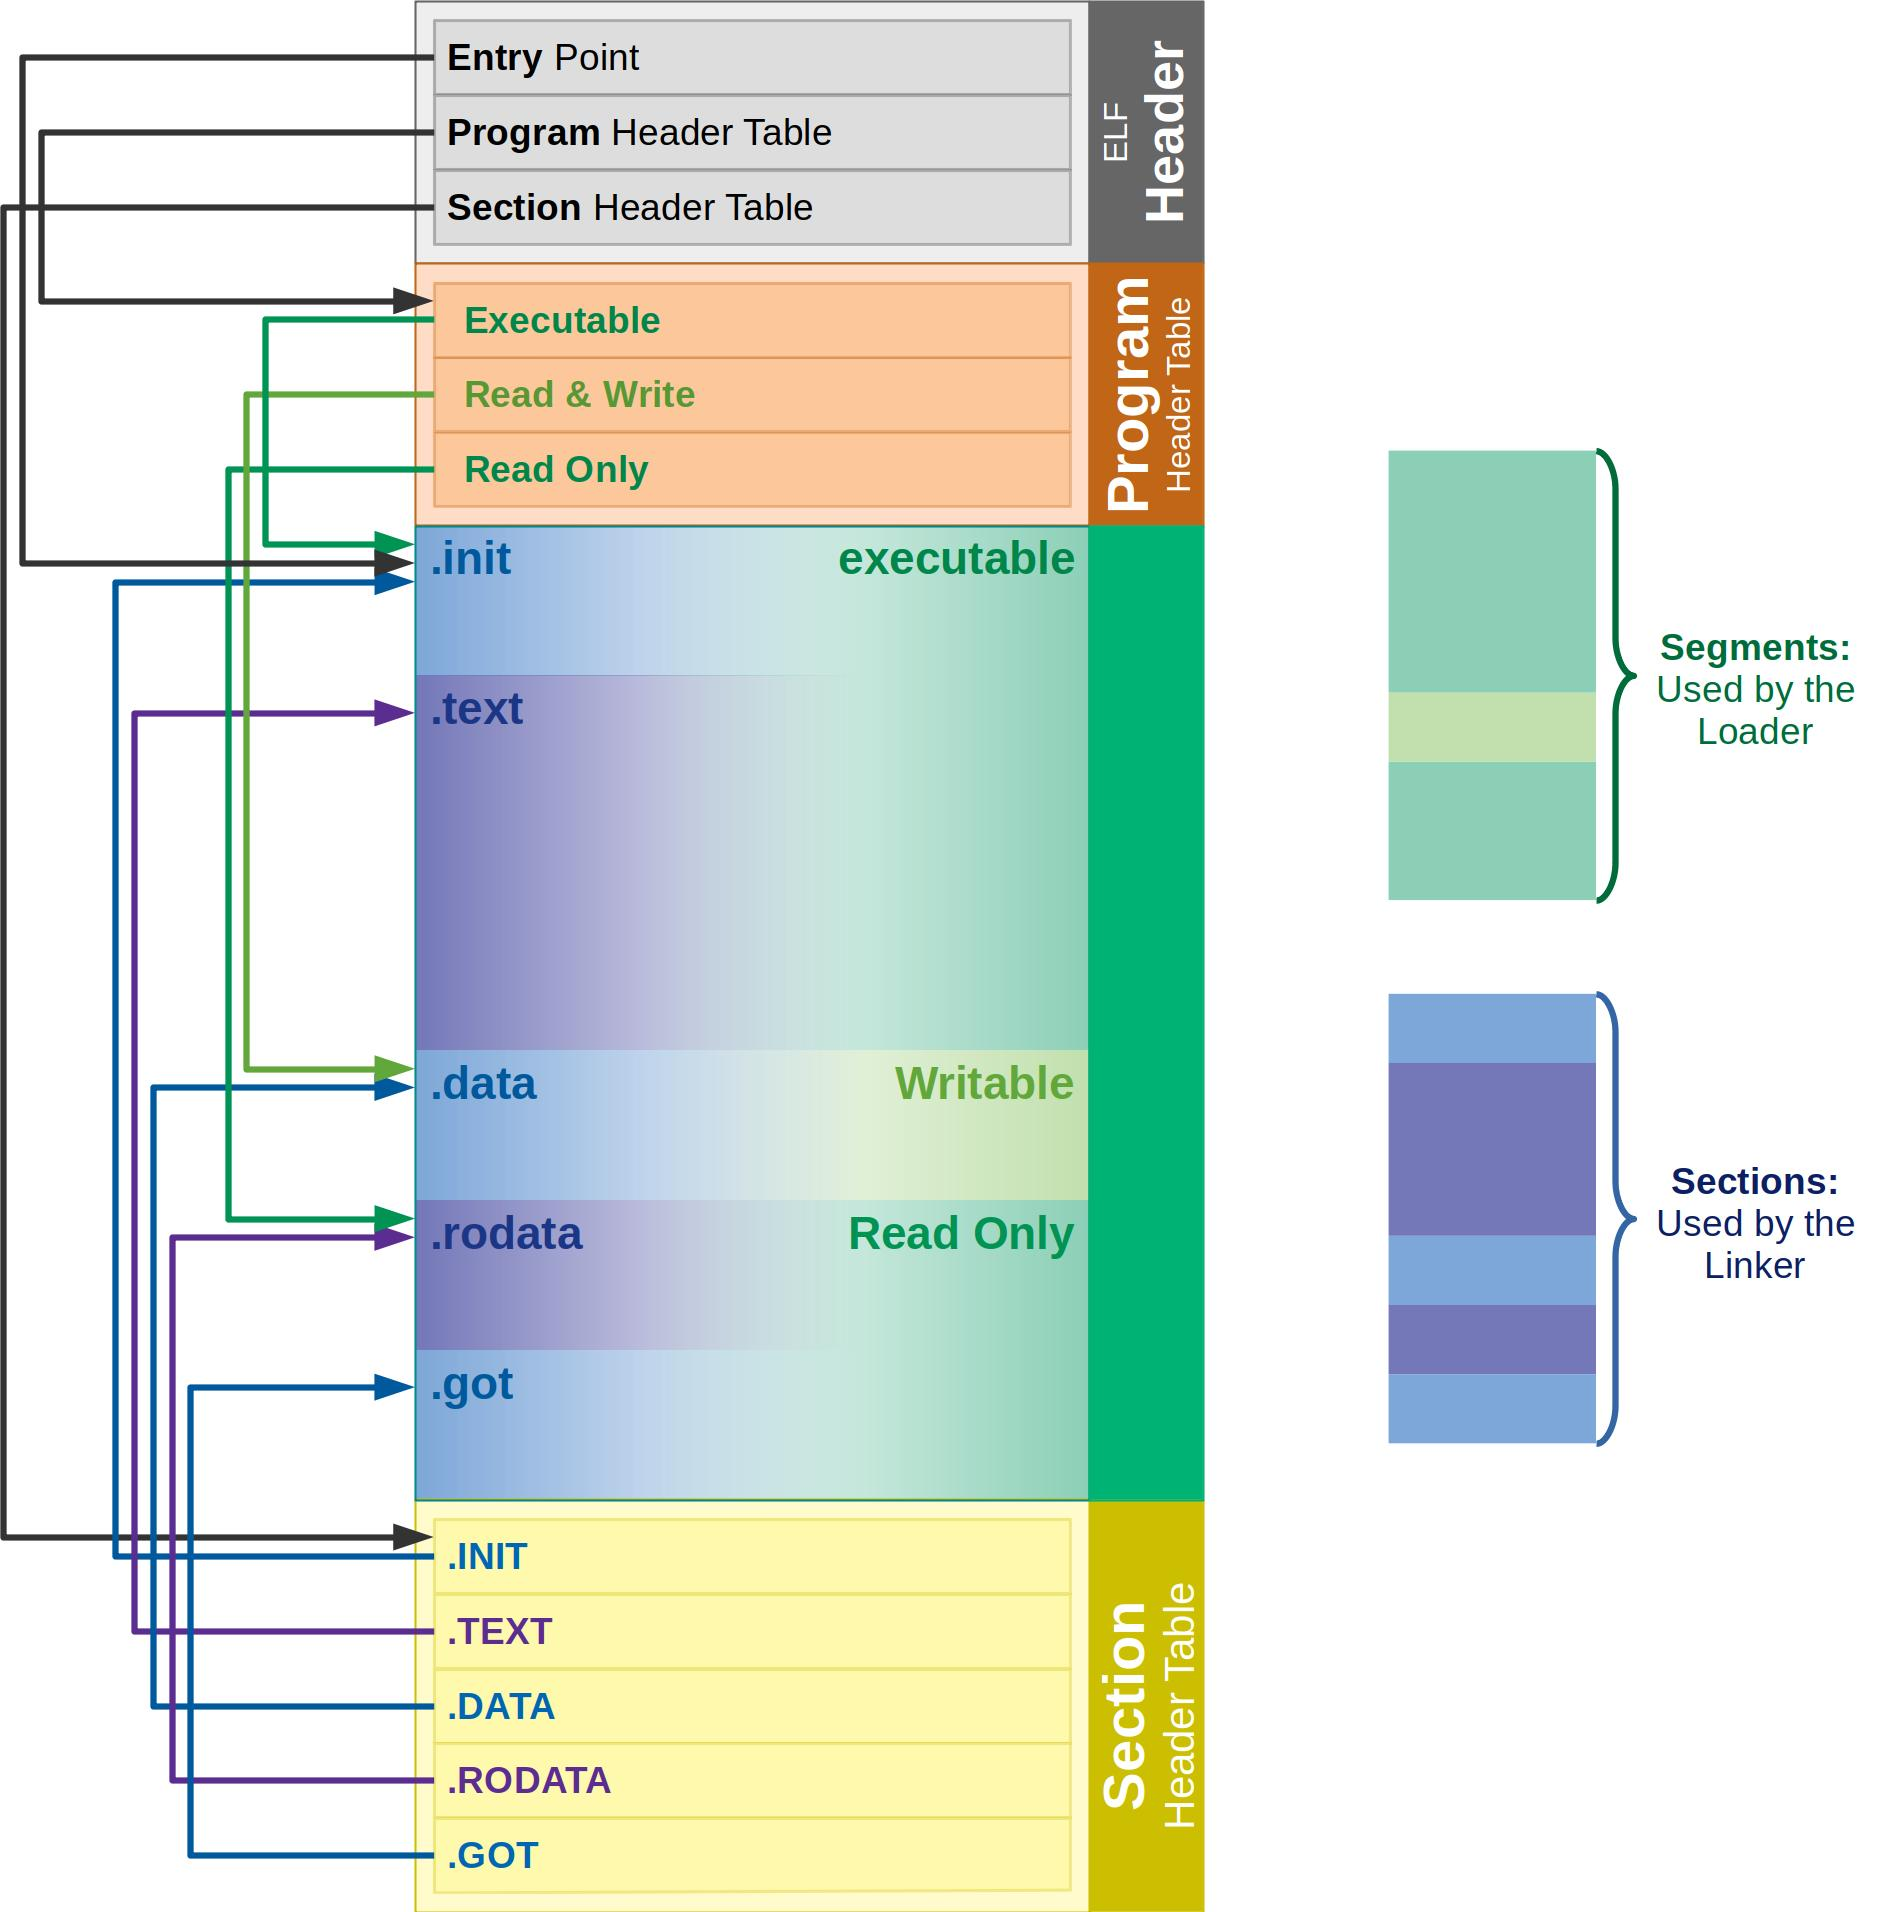
\includegraphics[width=300pt]{assets/typical_elf.jpg}
    \caption{Typical ELF file layout \cite{HW3238POperating}
    .}
    \label{fig:elf-layout}
\end{figure}


    \begin{minted}{text}
    $ fq .header /usr/bin/ls
        |00 01 02 03 04 05 06 07|01234567|.header{}:
    0x00|7f 45 4c 46 02 01 01 00|.ELF....|  ident{}:
    0x08|00 00 00 00 00 00 00 00|........|
    0x10|03 00                  |..      |  type: "dyn" (0x3)
    0x10|      3e 00            |  >.    |  machine: "x86_64" (0x3e)
    \end{minted}


An ELF file composed of a headers, which contains some
metadata about the file itself, segments containing the
actual code and some more metadata at the end. For the scope
of a package manager, it is of interest the study of this
data that is store on an ELF. It is also important to note
that there are two types of executable ELF's:

\begin{itemize}
    \item Statically linked executables
    \item Dynamically linked executables
\end{itemize}

Statically linked executable are usually not distributed by
Linux operating systems. A static executable bundles every
link-time dependency, such that everything is contained in a
single file. So from a distributor's point of view, it
doesn't make sense to make every file bundle every single
dependency, as they could be shared by other components of
the operating system. And some libraries even harder to
statically link, sometimes making it impossible in practice.

Dynamically linked executables and libraries, on the other
hand, rely on parts of the ELF metadata to be able to
discover other dependencies. When a executable is loaded,
via the |exec| system call, the following (non-exhaustive) steps are
performed by the kernel:

\begin{itemize}
    \item The kernel reds the \acl{PHT} which contains
    |INTERP|, this is the requested interpreter for the
    binary.
    \begin{minted}[breaklines]{text}
$ eu-readelf -l /usr/bin/ls
Program Headers:
  INTERP         0x000318 0x0000000000000318 0x0000000000000318 0x00001c 0x00001c R   0x1
        [Requesting program interpreter: /lib64/ld-linux-x86-64.so.2]
  ...
    \end{minted}
    \item Control is transfered to the loader, in this case
    |ld-linux-x86-64.so.2| .
    \item The loader then looks into a different section:
    the |.dynamic|
    \begin{minted}[breaklines]{text}
$ eu-readelf -d /usr/bin/ls
Dynamic segment contains 24 entries:
 Addr: 0x0000000000021a98  Offset: 0x020a98  Link to section: [ 7] '.dynstr'
  Type              Value
  NEEDED            Shared library: [libselinux.so.1]
  NEEDED            Shared library: [libc.so.6]
...
\end{minted}
    \item For each |NEEDED| library, the loader opens it and
    performs the symbol relocations to load them into
    memory.
    \item Finally, the control is transferred into the
    |_start| symbol, which performs some actions and then
    loads the |main| function for a C program.
\end{itemize}

This link loader (also known as dynamic linker) is part of
libc, one of the most important libraries in a Linux
operating system, that provides the standard C library. What
is important from the package manager's perspective, is how
ld-linux loads the dependencies for the |NEEDED| sections.
The manual page for |ld.so| \cite{LdLinuxManual} explains
the following behavior:

\begin{minted}[breaklines]{text}
If a shared object dependency does not contain a slash, then it
is searched for in the following order:

o  Using the directories specified in the DT_RPATH dynamic
   section attribute of the binary if present and DT_RUNPATH
   attribute does not exist.  Use of DT_RPATH is deprecated.

o  Using the environment variable LD_LIBRARY_PATH, unless the
   executable is being run in secure-execution mode (see below),
   in which case this variable is ignored.

o  Using the directories specified in the DT_RUNPATH dynamic
   section attribute of the binary if present.  Such directories
   are searched only to find those objects required by DT_NEEDED
   (direct dependencies) entries and do not apply to those
   objects' children, which must themselves have their own
   DT_RUNPATH entries.  This is unlike DT_RPATH, which is applied
   to searches for all children in the dependency tree.

o  From the cache file /etc/ld.so.cache, which contains a
   compiled list of candidate shared objects previously found in
   the augmented library path.  If, however, the binary was
   linked with the -z nodeflib linker option, shared objects in
   the default paths are skipped.  Shared objects installed in
   hardware capability directories (see below) are preferred to
   other shared objects.

o  In the default path /lib, and then /usr/lib.  (On some 64-bit
   architectures, the default paths for 64-bit shared objects are
   /lib64, and then /usr/lib64.)  If the binary was linked with
   the -z nodeflib linker option, this step is skipped.
\end{minted}

Usually for a conventional Linux distribution, the last
option is the most transversed. That is, loading file from
the default search path in |/usr/lib| or |/lib|. However,
for the software deployment model proposed in the previous
sections, packages don't link again the default search path,
as this causes the issues already explained.
|/etc/ld.so.cache| is also a shorthand for adding
globally-available libraries into the search path.

Finally, what the ELF format provides is the |RUNPATH|
section, which is searched for libaries contained in the
|NEEDED| sections. This |RUNPATH| is very useful, as it
allows every single binary file, to know where to look for
its own hashed dependencies. The link loader can also be
changed to a specific version, instead of relying in a
global |ld-linux.so|. This is done by changing the
|INTERP| in the \ac{PHT}.


As an alternative to a global search path such as the
following layout:

\begin{minted}{text}
INTERP   /lib/ld-linux.so.6
NEEDED   Shared library: [libc.so.6]
RUNPATH  -
\end{minted}

The following layout for an ELF file can be constructed:

\begin{minted}{text}
INTERP   /miq/store/libc-hashAAA/lib/ld-linux.so.6
NEEDED   Shared library: [libc.so.6]
RUNPATH  Library runpath: [/miq/store/libc-hashAAA/lib]
\end{minted}

With a modification of the ELF file metadata, then it is
possible to have a file load exactly the dependencies that
are computed at build time, to support the deployment model
discussed previously. The following chapter describes how
this modification of the ELF metadata is performed.

\FloatBarrier
\section{Other file types}

Not every file in a Linux system is an binary (ELF) file
however. A common Linux system is composed of many ``glue''
shell scripts, or any other text-based file. These files,
also perform the same ``dependency resolving'' that is done
in an ELF, but in a different way. For example, a shell
script that contains the following content:

\begin{minted}{sh}
#!/bin/sh

for file in /srv/backup/*; do
    cp $file /srv/backup2/
    chmod 600 /srv/backup2/$file
done
\end{minted}

A shell script like this also performes another type of
dependency resolution at run-time: loading any existing
program from |PATH|. In this case, both the |cp| and |chmod|
programs are external to the script, and also implicitely
dependencies of itself. For a toy script, it is easy to
underestimate this type of dependency resolution (as |cp|
and |chmod| are included in every Linux distribution), but
as scripts grow bigger, with more and more dependencies, it
becomes hard to keep track of every package.

The first line contains the |#!| sequence, which is called a
``shebang''. Analgous to the ELF format and |ld-linux|, the
shebang instruct Linux to load the program in this path, and
pass the rest of the file into it for execution. In turn
``sh'', interprets the rest of the file as a shell script,
and when faced with the |cp| and |chmod| commands, it reads
the environment variable |PATH|. This is also analogous to
the |RUNPATH| section of a ELF file, but contains
directories with executables:

\begin{minted}[breaklines]{text}
$ printenv PATH | tr ':' '\n'
/usr/local/sbin
/usr/local/bin
/usr/sbin
/usr/bin
/sbin
/bin
/usr/games
/usr/local/games
/usr/lib/wsl/lib
/snap/bin
\end{minted}

These folders are scanned sequentially, until the first
match is found -- that is |/usr/local/sbin/cp|, |/usr/local/bin/cp|, etc.

To avoid this kind of ``implicit'' dependency resolution,
one could also try to use the same technique used for ELF,
namely changing the |RUNPATH|. Unfortunately, this is not
possible, as scripts don't contain any extra ``metadata''
attached to them. A different solution is to construct a
shell script that contains full paths into the required
programs, and their full hashed paths in the store:

\begin{minted}{sh}
#!/miq/store/sh-version-hashAAA/bin/sh

for file in /srv/backup/*; do
    /miq/store/coreutils-version-hashAAA/bin/cp $file /srv/backup2/
    /miq/store/coreutils-version-hashAAA/bin/chmod 600 /srv/backup2/$file
done
\end{minted}

Doing these modifications is not as seamless as tweaking some
compile and link flags for an ELF file, and an automation
tool would be required to resolve the implicit dependencies
of a shell script.

The list of language-specific tweaks would continue -- for
example |PYTHONPATH| for Python packages -- but for the sake
of simplicity, only shell scripts and binary ELF files are
considered in this project. Usually each language ecosystem
has each own method of dependency resolution that can be
overriden to not use a ``global'' search path.

\FloatBarrier
\section{Base Linux packages}

To understand the scope of a Linux package manager, we need
to define what constitutes a Linux operating system. To
answer this question, we can take a look at the past, on the
inception on Linux. We can trace back to the UNIX system
\cite{ritchieUNIXSystemEvolution1984} developed by Ken
Thompson, Dennis Ritchie, and others. This operating system
marked a milestone in the history of computing, and the work
of its authors could be divided into 2 research fields: the
development of the interfaces of the OS, and a new
programming language to accompany it, the C programming
language. The UNIX kernel was rewritten in this new
language, and in 1978, the book
``The C Programming Language''
\cite{ritchieProgrammingLanguage1983} was
released, setting the foundation of the language into the
future. As UNIX started to gain popularity, the project
increasingly started to lock users in. As an alternative to
UNIX, the GNU (GNU is Not Unix) project started with the
intention to provide a UNIX-compatible operating system that
would not lock users in with proprietary software licenses.
Finally, the Linux kernel was created by Linus Torvalds
around 1991 as a research project to provide a substitute to
the MINIX kernel, and finally the GNU components replaced
any leftovers of MINIX \cite{OverviewGNUSystem}.

The Linux kernel and all of the GNU components were written
in C, so it became the de-facto language for system
software. Therefore, the C language is intertwined with how
a Linux operating system works, and all the packages that
compose it from the kernel to userland. From the packager's
perspective, there is one package that is the most
important: \textbf{libc}. The C standard library (libc, or
GNU's libc implementation, glibc) is a collection of C
headers and library objects that provide interfaces to the
operating system for programs written in C. Libc was
standardized in 1999 by the ISO C committee under the C99
language specification, and further revisions were made to
update it. Some of the headers from libc include:

\begin{figure}[hbt]
    \centerfloat
    \begin{tblr}{hlines, vlines}

        <string.h> & String manipulation \\

        <stdio.h> & Standard input/output \\

        <stdint.h> & Standard integer types \\

        ... & ... \\

    \end{tblr}
    \caption{Some of the headers from libc.}
\end{figure}

For Linux, there are various implementations of libc, such
GNU's glibc or musl libc \cite{MuslLibc}, being the former
the predominant on all popular Linux distributions. Along
with the headers required by the C ISO standard, the libc
providers are implemented over the kernel's system calls and
also provide UNIX-specific interfaces, namely |<unistd.h>|.
Libc is also the provider of the link-loader discussed in
previous sections (ld-linux.so), and also injects some
loading code in every ELF file, before the main function
execution takes over.

Apart from libc, many programs and libraries are implemented
on top of it, to provide what is called as the \acl{LSB}
\cite{LinuxStandardBase} . This specification outlines some
of the most important programs that compose a Linux system,
such as ``coreutils'', which contains the most basic
terminal utilities, like |ls|, |cat|, |cp|, etc. To be able
to build the components, it is also needed a C compiler,
which is also provided by the GNU project in form of GCC
(GNU Compiler Collection). To
be able to support the compilation and configuration of
programs, some other tools are required like |make| or
|sed|, and also a POSIX shell to interact with the system,
in the form of |bash|. The table \ref{tab:lsb} outlines some
of these componentes and their functionality.

\begin{figure}[hbt]
    \centerfloat
    \begin{tblr}{hlines, vlines}
        libc & C standard library (glibc, musl) \\

        gcc & C and C++ compiler \\
        coreutils & Basic terminal utilities, like ls,
        cat, cp, etc. \\
        binutils & Binary utilities, like ld, as,
        objdump, etc. \\
         make & Build automation tool \\
         sed & Stream editor, text modification
        program \\
         bash & POSIX shell implementation \\
         tar & Archive utility \\
         grep & Text search utility \\
         findutils & File search utilities, like
        find or findmnt \\
         diffutils & File comparison utilities, like
        diff \\
         systemd & System and service manager \\
    \end{tblr}
    \caption{Some of the basic components of a Linux system.}
    \label{tab:lsb}
\end{figure}

As a Linux distribution grows in scope, more and more
components are needed to build something that an end-user is
able to use. Starting from graphical toolkits, like GTK or
QT, to the X11 display server and desktop environments, like
Gnome or KDE Plasma. And every component in-between, like
proper service management via systemd, the package manager
itself, network management, power management, peripherals
support, and all the libraries that are required to build
all the ``leaf'' packages of the full dependency tree.
Finally, the kernel itself is also a package with special
properties (as it doesn't depend on libc), but regardless of
importance.

The scope of this work has been limited to a basic terminal
usage of Linux packages, so the focus won't be on building
complex software, but rather building basic components to
prove the viability of the deployment model. It is also
important to note, that while packages can be put together
to form a fully function independent operating system, a
package manager of Linux packages can work as a ``guest'' on
a different distribution. This is, running Linux packages
that are not part of the distribution itself. For a
classical system, this has never been common practice -- for
example, installing apt (Debian's package manager) on a
Gentoo system -- mainly limited by the rules imposed by the
\acl{FHS}. Basically, two package managers would interfere
with each other, as they would try to manage files that were
managed by the other package manager (any file on /usr/bin,
/usr/lib, etc). However, with the usage of the special
hash-based paths, this problem not an issue, as miq can be
used on top of any Linux distribution, without interfering
with it.

\FloatBarrier
\section{The bootstrapping problem}

As discussed in the previous section, the scope of this work
is to be able to demonstrate the viability of the deployment
model of hashed paths instead of relying in the \ac{FHS}.
So, as one of the core libraries, libc is the one to be
compiled the first. As mentioned previously, libc is the C
standard library, that in practice is used by every program
written in C, which make up the core programs of a Linux
operating system. To be able to compile libc, it is required
a C compiler (from GCC), a POSIX shell (bash, for
example) and other utilities. In this project, musl libc was used instead of
glibc, as GNU's version contains some extra additions that
are not part of the standard, which could introduce
complexity. Then, a dependency graph for musl libc can be
drawn as shown in figure \ref{fig:libc-deps}.

\begin{figure}[hbt]
    \centerfloat
    \includesvg[width=150pt]{graph/libc-bs1.dot.svg}
    \caption{Dependency graph for musl libc on first iteration.}
    \label{fig:libc-deps}
\end{figure}

These GCC dependency in this graph is assumed to already
"exist" in the system. But as already discussed, this is a
source of impurity, as we don't know what C compiler was
used, we can't hash the input to produce a hash for the musl
output. This C compiler is ``external'' to the system.
Therefore one of the objectives of any package manager is to
be able to ``support'' itself, to be able to produce
packages without any external interference. Then, this GCC
must come from the package manager itself as well, and we
can draw its dependency graph in figure \ref{fig:libc-deps2} .

\begin{figure}[hbt]
    \centerfloat
    \includesvg[width=200pt]{graph/libc-bs2.dot.svg}
    \caption{Dependency graph for musl libc on second iteration, recursive nature shows.}
    \label{fig:libc-deps2}
\end{figure}

As can be seen, to be able to build libc, we need a C
compiler, and to build a C compiler we need libc. This is a
problem of a circular dependency, in particular the
bootstrapping problem, because we need to ``base'' to be
able to lift the entire system system from the ground.
Moreover, if we try to draw a dependency from cyclically as
in figure \ref{fig:libc-deps3}, we can see that graph is now
\emph{cyclic}, this means that it is no longer a \ac{DAG} as
discussed in the previous section, and we can no longer hash
the nodes, as it would result in a infinite recursion. For
this reason, cyclic dependencies are not allowed in miq, and
using and checking for a proper \ac{DAG} is important.

\begin{figure}[hbt]
    \centerfloat
    \includesvg[width=150pt]{graph/libc-bs3.dot.svg}
    \caption{Cyclic dependency graph for musl libc and gcc.}
    \label{fig:libc-deps3}
\end{figure}

To solve the bootstrapping problem, a solution is proposed
of providing a set of bootstrap tools. This set of tools is
downloaded from the internet, ready to use. By using it as a
``fixed hash'' package, we can break the chain of recursive
dependencies, as shown in figure \ref{fig:libc-deps4}. This
set of bootstrap tools doesn't need to be updated ever. For
example, they could contain a very old GCC, such that it is
recent enough to be able to compile a newer GCC used for the
rest of the packages on the system.

\begin{figure}[hbt]
    \centerfloat
    \includesvg[width=150pt]{graph/libc-bs4.dot.svg}
    \caption{Dependency graph for musl libc with a loop on gcc, solved with a bootstrap package.}
    \label{fig:libc-deps4}
\end{figure}

In practice, the Linux distributions don't use the first
iteration of this process. Instead, an iterative process is
created, where libc and the C compiler (along any extra
tools) are compiled in succession, using the result of the
previous step to compile the next one. These are called
``stages'', and the process ``distills'' the programs until
an stable result is obtained. The final stage (from 0 to 1,
2 , etc) is then used to build the system, instead of the
zero-th stage.

\begin{figure}[hbt]
    \centerfloat
    \includesvg[width=200pt]{graph/libc-bs5.dot.svg}
    \caption{Bootstrap tower with 3 stages.}
    \label{fig:libc-deps5}
\end{figure}


\section{GNU Autotools}

\FloatBarrier
\chapter{Implementation}

The following chapter describes the implementation of miq.
Miq is the program that was developed as a proof of concept
of the topics described in this document. As such, miq
(pronounced [miku]), is a package manager for Linux. It can
be categorized as a ``source-based'' package manager,
because the user would build every package from its sources
(for example, Gentoo's package manager |emerge| or |nix|),
as opposed to to a ``binary-based'' package manager, which
distributes the already-built packages to its users.

The model of a source-based package manager provides some
advantages, such as being able to edit the recipes that
build the packages. Moreover, by integrating the tool that
builds the packages and the tool that installs them, the
user gets a fast feedback loop to iterate over the writing
of the package definitions. In a source-based package
manager, the user receives a copy of a source tree that
contains the recipes, definitions of all the packages in the
repository. These files contain the instructions about all
the packages that are available, and the machine-readable
data for the package manager to build them. The user would
tell the package manager to build or install certain package
X, and the program would then:

\begin{itemize}
    \item Evaluate the file tree of package definitions.
    \item Calculate a transaction (which files to build or download)
    \item Perform the transaction
\end{itemize}


miq is heavily inspired by nix, the functional package
manager, a work of \Citeauthor{dolstraNixOS2008}
\cite{dolstraNixOS2008}. The work of nix of using a
hash-based path system instead of the \ac{FHS} was the idea
that lead this project, and that is implemented in miq by
following the same conventions that in nix. This means, that
packages are configured with a custom prefix that lives in
the \textbf{store} (|/miq/store| and |/nix/store| respectively), with
a unique subdirectory based on the hash of the package
definition -- which implies that any change in its
dependencies would trigger a recalculation of the store
path. Miq differs with nix in that the schema for the
calculation of the store path follows the pattern
|name-version-hash|, while nix uses |hash-name-version|.
While the result of the package is functionally the same, by
using the name first, the list of folders in |/miq/store|
can be easily ordered by package name.

Miq differs from nix in the usage of the language used for
the evaluation of the packages. On of the powerful features
of both miq and nix is the ability to declare packages as
code, using a turing-complete programming language. This is
in contrast to apt or rpm, which use a markup language to
define the packages. By using a turing-complete language,
the user is able to create any kind of abstraction around
the package primitives. This not only allows for code
deduplication, but also to easily create new ``helper''
packages that would otherwise not be considered with a
classical markup-language based package manager.

In this regard, for nix, a new programming language was
invented with the same name, nix. This is a purely
functional language inspired by the semantics of Haskell, and
often referred to as ``JSON with functions''. As this
language is sometimes alien to users, with miq the decision
was to use Lua, an easily emendable language. This is
discussed in more depth in section \ref{sec:lua} .

Miq is implemented in the Rust programming language
\cite{RustProgrammingLanguage} . Rust is a relatively new
language created at Mozilla, which focuses on the ability to
build fast and reliable programs. This is achieved through
the use of rich type system, that guards the programmer from
making mistakes and eases the process of a refactor. Rust
also provides some other features that were viable to this
project. A very important detail is that Rust can build
native binaries (ELF) that can be run by the operating
system. Every dependency of the Rust program (crates) are
also built into the final binary, and C library requirements
(libc) are statically linked. This means that the final
result is a single |20MB| binary, with no dependencies that can be
run in any Linux system, no matter the distribution.

\section{Units: the basic building blocks}

The main purpose of the package manager, is to build
packages according to a dependency tree. Therefore, it is
important to properly define what a ``package'' is and is
not. In miq, the concept of a package has been abstracted by
the concept of a ``unit''. A unit is something that can be
built, and put into the miq store (|/miq/store|). This
abstraction has been chosen, because it makes it easy to
have different entities that can be built. This
differentiation serves the purpose of being able to declare
2 types of units: package units, and fetchable units.
As discussed in section \ref{sec:builder}, package units are
built in a network sandbox, to avoid impurities resulting of
a connection to the network. The main aspect of miq is being
able to hash packages depending on its dependencies and
build script. The ``result'' of building the package is not
considered in the hashing algorithm. This can be described
as packages being input-addressed, instead of
content-addressed. As such, it is important to have a proper
build sandbox to isolate the build process and produce a
reproducible result, for the same input parameters. The
purpose of fetchable units (|Fetch|) is to be able to split
the network connection from the build process. The
implementation for |Unit| is a enumeration with 2 cases:

\begin{minted}{rust}
#[derive(Clone, Debug, Serialize, Deserialize, Hash)]
enum Unit {
    PackageUnit(Package),
    FetchUnit(Fetch),
}
\end{minted}

This example already shows one of the features of Rust that
made the development of miq ergonomic: |derive| macros.
|derive| is a keyword that allows for automatic code
generation given some |struct| or |enum|. In this case the
|Hash| trait is derived. What this means is that Rust
automatically generates an implementation for the |Hash|
trait, given that the fields of the enum are also |Hash|.

Very importantly too, the traits |Serialize| and
|Deserialize| are derived for Unit. These traits are
provided by the |serde| crate (serialization and
deserialization) \cite{Serde} . Similarly to the |Hash|
derive macro, serde allows to automatically generate
serialize and deserialize a Unit from any crate that
provides an interface for it. This comes into play for the
usage of the intermediate representation objects that are
store into disk, in |toml| format. As discussed in the next
section, miq loads the units from disk in |toml| format, and
automatically parses them into the data structure, without
any need of parsing code.

The Unit enum has two members, which wrap the inner values:
|Package| and |Fetch|. These are structs that contain all
the information that miq uses to build the Unit. The
implementation of the Fetch unit is trivial, as the
following code snippet shows:

\begin{minted}{rust}
#[derive(Deserialize, Serialize, Hash)]
struct Fetch {
    result: MiqResult,
    name: String,
    url: String,
    executable: bool,
}
\end{minted}

The toml format is an human-readable serialization format,
that can be compared to JSON. As the latter is not
considered ergonomic to manually write, it was decided to
use the toml format instead, although this doesn't have any
impact on the functioning of the package manager. The
following snippet of code shows a serialization of the musl
Fetch Unit.

\begin{minted}{toml}
# /miq/eval/musl-1.2.3.tar.gz-828bf8f78328fb26.toml
type = "FetchUnit"
result = "musl-1.2.3.tar.gz-828bf8f78328fb26"
name = "musl-1.2.3.tar.gz"
url = "https://musl.libc.org/releases/musl-1.2.3.tar.gz"
executable = false
\end{minted}

The example above already shows the hashing of the Unit
itself: the |result| field. This field is computed as a
function of the |url| and the |executable| fields, and
determines the hashing of the Unit itself. This is stored
attached to the Unit itself. This example is trivial, but
any other Fetch unit with the same |name|
(|musl-1.2.3.tar.gz|) but different |url|, would trigger a
change in the hashing that ends up in |result|, as shown in
figure \ref{fig:fetch_hash} .

\begin{figure}[hbt]
    \centerfloat
    \includesvg[width=350pt]{assets/fetch_hash.svg}
    \caption{Hashing process of a Fetch Unit.}
    \label{fig:fetch_hash}
\end{figure}

Similarly, a Package Unit is written as a struct with the
instructions required to build it. The following simplified
snippet shows the implementation in Rust:

\begin{minted}{rust}
#[derive(Serialize, Deserialize, Hash)]
pub struct Package {
    result: MiqResult,
    name: String,
    version: Option<String>,
    deps: BTreeSet<MiqResult>,
    script: String,
    env: BTreeMap<String, String>,
}
\end{minted}

An example serialization of a Package Unit for musl is the
following:

\begin{minted}{toml}
# /miq/eval/musl-f0dd14ee1ca91c64.toml
type = "PackageUnit"
result = "musl-f0dd14ee1ca91c64"
name = "musl"
version = "1.2.3"
deps = [
    "musl-1.2.3.tar.gz-unpack-5f9d5116c4c83592",
    "stage0-stdenv-d2ecc89c54b1b316",
]
script = '''
source /miq/store/stage0-stdenv-d2ecc89c54b1b316/stdenv.sh
set -ex
/miq/store/musl-1.2.3.tar.gz-unpack-5f9d5116c4c83592/configure \
    --prefix=$PREFIX \
    --disable-static \
    --enable-wrapper=all \
    --syslibdir=$PREFIX/lib
make -j$(nproc)
make -j$(nproc) install
ln -vs $PREFIX/lib/libc.so $PREFIX/bin/ldd
'''
\end{minted}

A Package Unit is more complex than a Fetch Unit, because of
the following:
\begin{itemize}
    \item Package units have a |deps| field. |deps| are the
    |result| strings of any other Unit. This means Package
    Units can depend on other Package or Fetch Units, while
    Fetch Units don't depend on anything.
    \item The |build| field is a literal bash script that is
    used during the build process to produce the output.
\end{itemize}

In contrast to other package managers and similarly to nix,
miq doesn't provide multiple stages for the build process.
In Gentoo, the definition of package, usually contains some
unpack, build and install phases. In contrast, everything in
miq is done through the script section. This is because, by
using a language to generate this |toml| representation, the
user is free to include any custom functionality as needed.
This is important, as the Package Unit tries to be as
minimal as possible, by just providing the |script| phase,
and letting the user construct any abstraction on top of it.
In the example, musl depends on |stdenv|, which is a script
that sets some environment variables required for the build
process, effectively implementing the concept of build
stages in other package managers.

\begin{figure}[hbt]
    \centerfloat
    \includesvg[width=350pt]{assets/phash.svg}
    \caption{Hashing process of a Package Unit.}
    \label{fig:pkg_hash}
\end{figure}

The hashing algorithm used for the process is the
\textit{Fowler Noll Vo} hash function \cite{FnvRust}. While
this algorithm is not cryptographically secure, and doesn't
provide protection against collision attacks, the algorithm
could be considered as sufficient for this application. This
could be considered as an implementation detail, and could
be swapped for any algorithm such as |SHA256| if deemed
necessary.

The implementation of miq uses a 2-stage evaluator, that
first converts the Lua code into a serialization of Units,
and then serializes them again to sort the dependency
algorithm. Unit files are stored in the |/miq/eval|
directory, generated and consumed by miq in sequence, as
shown in figure \ref{fig:2stage} .

\begin{figure}[hbt]
    \centerfloat
    \includesvg[width=400pt]{assets/22stage.svg}\
    \caption{Two-staged evaluation process.}
    \label{fig:2stage}
\end{figure}

The purpose of this 2-stage evaluator process, is be able to
extend miq as needed. Because the |unit.toml| format is
well-known, a user or contributor should be able to
implement a different evaluator in any other language than
Lua. This is one of the main shortcomings of nix, as it
only allows the usage of the nix language. The Guix package
manager \cite{courtesFunctionalPackageManagement2013}
studied the usage of Scheme as the language for the
evaluation process, by patching into the nix builder. By
explicitly allowing for an intermediate format, the
ergonomics of the package manager could be improved.

As a side-effect of this design, some characteristics
emerge:

\begin{itemize}
    \item Units toml files can be manually written by hand.
    During the development process of miq, the Lua evaluator
    was the last piece implemented, because Unit files could
    be manually written as a proof of concept.
    \item Units can be copied and pasted from one machine to
    another. If the reproducibility of the evaluator cannot
    be assured, unit files can be checked out into version
    control. A user could then use the locally downloaded
    unit tree to build the resulting packages. This could be
    useful as an alternative distribution method to the Lua files.
\end{itemize}

\section{Dependency solver}

\section{Recipe evaluator}
\label{sec:lua}

\section{Builder}
\label{sec:builder}

\section{Database}





\chapter{Conclusions}
Test
\lipsum[20]


\newpage
\addcontentsline{toc}{chapter}{Bibliography}
\printbibliography[title=Bibliography]


\begin{titlepage}
  \addcontentsline{toc}{chapter}{List of Figures}
  \listoffigures

  % \listoftables

  \newpage
  \addcontentsline{toc}{chapter}{Acronyms}
  \chapter*{Acronyms}
    \begin{acronym}
        \acro{DAG}{Directed Acyclic Graph}
        \acro{FHS}{Filesystem Hierarchy Standard}
        \acro{CLI}{Command Line Interface}
        \acro{HPC}{High-performance computing}
        \acro{VM}{Virtual Machine}
        \acro{OS}{Operating System}
    \end{acronym}
\end{titlepage}

% \chapter{Annexes}
\chapter{Annexes}

\section{Miq installation}

Miq is an open-source project written in Rust. This allows
to easily build the project into a single executable that
bundles all its dependencies. The only C dependencies (libc
and sqlite3) are statically linked too.

By using GitHub actions, the latest version of the project
is compiled and pushed into the ``releases'' section of the
repository. It is only built for |x86_64| Linux machines.

To download the latest version of the project, follow the
following instructions:

\begin{enumerate}
    \item Download the release tarball, containing the
    executable itself, a copy of Bubblewrap and the Lua
    files that describe the packages, optionally changing to
    some new directory:
\begin{minted}{text}
$ mkdir ~/miq && cd ~/miq
$ curl -OL https://github.com/viperML/miq/releases/download/latest/release.tar.gz
\end{minted}

    \item Extract the tarball:
\begin{minted}{text}
tar -xvf release.tar.gz
\end{minted}

    \item Add the current directory to |PATH|, such that
    |bwrap| can be found (this can be skipped if the host
    machine has Bubblewrap installed):
\begin{minted}{text}
$ export PATH="$PWD:$PATH"
\end{minted}

    \item Miq is ready to be used
\begin{minted}{text}
$ miq --help
miq 0.1.0
Fernando Ayats <ayatsfer@gmail.com>

Usage: miq <COMMAND>

Commands:
    build   Build a package
    eval    Evaluate packages
    lua     Reference implementation of the evaluator, in Lua
    store   Query the file storage
    schema  Generate the IR schema

Options:
    -h, --help     Print help
    -V, --version  Print version
\end{minted}

\end{enumerate}




\section{Miq usage manual}

The following subsections describe the usage of the \ac{CLI}
of miq. While short descriptions can be accessed through the
|--help| flags for every subcommand, this document goes into
more detail about each function.
Miq should have been installed according to the instructions
in the previous section.

As discussed in chapter
\ref{chap:overview}, miq is composed of 4 main components: a
2-stage evaluator, the builder and the database handler,
displayed in figure \ref{fig:miq-components}. These
components can be accessed sequentially, by using the
appropriate subcommands.

\subsection{Evaluating packages}
\label{sec:eval}

The most basic function of miq is to only run the package
evaluator. The packages are described in Lua files, which
are run and produce a dependency graph in memory. The
evaluator can be run separately without building any
package, and performs the two stages:

\begin{enumerate}
    \item Run the Lua code, which produces intermediate
    representation Unit files in |/miq/eval/*.toml| .
    \item Parse the Unit files and calculate the
    dependencies between them to produce a dependency \ac{DAG}.
\end{enumerate}

Step 1 can be skipped, if the user decides to use a
pre-evaluated toml file.

The entrypoint in the \ac{CLI} is the subcommand |miq eval|.

\begin{minted}{text}
$ miq eval --help
Evaluate packages

Usage: miq eval [OPTIONS] <UNIT_REF>

Arguments:
    <UNIT_REF>  Unitref to evaluate

Options:
    -o, --output-file <OUTPUT_FILE>  Write the resulting graph to this file
    -n, --no-dag
        --eval-paths                 Print eval paths instead of names
    -h, --help                       Print help
\end{minted}

|miq eval| takes a Unit reference. Currently there two types
of Unit references:

\begin{itemize}
    \item Serialized Unit reference. This is a direct
    reference to a Unit file |/miq/eval/*.toml|, which skips
    the Lua evaluator.
    \item Lua Unit reference. This reference has two parts
    separated by a hash symbol: |file.lua#item| .
\end{itemize}

Within the miq release tarball, it is distributed a set of
Lua files written for this project that can build some
applications. The main entry point of these files is
|init.lua| . The Lua file pointed by the \ac{CLI} must
return a table, of which it can be selected the key to
build (nested tables are supported, by using the syntax
|file.lua#parent.child|).

After evaluating a Lua file, miq would print any errors
encountered, or otherwise a |dot| language representation of
the \ac{DAG}, as the following example shows:

\begin{minted}{text}
$ miq eval ./init.lua#stage0.bootstrap
digraph {
    0 [ label = "bootstrap" ]
    1 [ label = "bootstrap-tools.tar.xz", shape=box, color=gray70 ]
    2 [ label = "busybox", shape=box, color=gray70 ]
    3 [ label = "toybox-x86_64", shape=box, color=gray70 ]
    4 [ label = "unpack-bootstrap-tools.sh", shape=box, color=gray70 ]
    0 -> 1 [ ]
    0 -> 2 [ ]
    0 -> 3 [ ]
    0 -> 4 [ ]
}
\end{minted}

This graph can be manually inspected to check if the result
matches the desired output. With the |dot| tool from the
|graphviz| package, this graph can be rendered into an
image, as shown by the following example:

\begin{minted}{text}
$ miq eval ./init.lua#stage0.bootstrap | dot -Tsvg > graph.svg
\end{minted}

\begin{figure}[hbt]
    \centerfloat
    \includesvg[width=300pt]{assets/example.svg}
    \caption{Example of a dependency graph produce by miq eval.}
    \label{fig:miq-eval-graph}
\end{figure}

Nodes with a dim boxed outlines are Fetch Units, while round
default nodes represent Package Units.


\FloatBarrier
\subsection{Lua API}

As mentioned in this project, miq uses Lua as a scripting
language to describe packages, instead of using |bash| like
some Linux distributions like Gentoo or Arch Linux, for their
ebuilds or PKGBUILDs respectively.

The Lua runtime is completely embedded into the miq
executable, and allows for a very ergonomic and powerful
interface between the scripting language and the Rust native
code.

The Lua evaluator takes a top-level Lua file, which must
return a Lua table. This table may contain any number of
key-value pairs of package names to its Units, but nested
tables are also allowed, as well as any other data type that
can be ignored. The Rust runtime inserts a library into the
available functions, so no Lua code is required to import
the standard library:

\begin{minted}{lua}
local miq = require("miq")
\end{minted}

The available functions are:

\begin{itemize}
    \item |miq.fetch|: Function that creates a Unit of kind
    Fetch. The input must be a table with the following
    keys:
    \begin{minted}{text}
url = <string> -- URL to fetch
executable = <bool> -- Wether to set the file as executable. Optional, default is false.
    \end{minted}

    \item |miq.package|: Function that creates a Unit of
    Package. The table input must contain the following
    keys:
    \begin{minted}{text}
name = <string> -- Name of the package
version = <string> -- Version of the package. Optional default is empty.
script = <string|MetaText> -- Bash script to execute during
build. May be the output of the f function.
env = <table> -- Environment variables to set during build. Optional.
\end{minted}

    \item |miq.f|: Function that takes a single string as
    input. The string is parsed looking for the characters
    |{{ }}|, and for every match, it substitutes the name of
    the variable, similar to how f-strings work in Python.
    |f| can substitute strings into strings, but also Units
    into strings. When a Unit is substituted into a string,
    a different value is returned: a MetaText. A MetaText is
    just a table containing the string with a list of
    dependencies.
    \begin{itemize}
        \item The string is the result of substituting the
        store path of the Unit .
        \item The list of dependencies gets appended the
        Unit that was substituted.
    \end{itemize}
    |f| also supports interpolating strings or Units into a
    MetaText.

    \item |miq.trace|: Function that takes any Lua value and
    logs it into console, by printing a pretty
    representation. Lua tables are usually printed by just
    the numeric representation of pointer into the heap,
    while |miq.trace| prints the table as a list of
    key-value pairs.
\end{itemize}

While Units are serialized into plain Lua tables that can be
manipulated by hand, it is advised to only use Units that
are produced by the API functions, as the Rust runtime
relies on the exact keys being present in the table.

On the other hand, a set of functions are implemented in
native Lua, that wrap the API functions, as short hands to
easily represent the packages. The functions are organized
into different files, which can be ``required'' by each
other or in the top level |init.lua|.

\begin{minted}{lua}
local utils = require("utils")
local stage0 = require("stage0")
local stage1 = require("stage1")
\end{minted}

Moreover, the list of packages is organized into different
``stages'', with the purpose of trying to build a C compiler
cleanly, by progressively building the tools required to do
so and using them into the next stage. These stages contain
examples of how packages may be implemented.


\subsection{Building packages}

To build a package, the command used is |miq build| :
\begin{minted}[breaklines]{text}
$ miq build --help
Build a package

Usage: miq build [OPTIONS] <UNIT_REF>

Arguments:
  <UNIT_REF>  Unitref to build

Options:
  -q, --quiet            Don't show build output
  -r, --rebuild          Rebuild the selected element, but don't rebuild its dependency tree
  -R, --rebuild-all      Rebuild all packages in the dependency tree
  -j, --jobs <MAX_JOBS>  Maximum number of concurrent build jobs. Fetch jobs are parallelized automatically [default: 1]
  -h, --help             Print help
\end{minted}

As discussed in the previous section \ref{sec:eval}, the
\ac{CLI} uses the concept of Unit references to either use a
raw toml Unit from |/miq/eval|, or to run a Lua script that
evaluates the necessary packages. With the same syntax as
|miq eval|, one can perform a build for a selected package:

\begin{minted}[breaklines]{text}
/miq/store/unpack-bootstrap-tools.sh-6949dd1f64cfe7b6 <- (Fetch { name: "unpack-bootstrap-tools.sh" },)
/miq/store/busybox-33a90b67a497c4d6 <- (Fetch { name: "busybox" },)
/miq/store/toybox-x86_64-69a4327d80d88104 <- (Fetch { name: "toybox-x86_64" },)
/miq/store/bootstrap-tools.tar.xz-9d678d0fc5041f17 <- (Fetch { name: "bootstrap-tools.tar.xz" },)
bootstrap>>+ /miq/store/toybox-x86_64-69a4327d80d88104 mkdir -p /build/bin
bootstrap>>+ export PATH=/build/bin:/no-such-path
bootstrap>>+ PATH=/build/bin:/no-such-path
bootstrap>>+ /miq/store/toybox-x86_64-69a4327d80d88104 ln -vs /miq/store/toybox-x86_64-69a4327d80d88104 /build/bin/ln
bootstrap>>'/build/bin/ln' ->
'/miq/store/toybox-x86_64-69a4327d80d88104'

...
\end{minted}

As builds are performed concurrently, the output shows a
prefix for the package that is outputting the log message,
displayed with |package>>|. After a Unit is built, its store
path is printed into the console, so that the output
contents can be manually inspected.

While Fetch jobs are automatically fetched in parallel,
Package Units are not by default, to be able to inspect the
logging messages properly. The user may want to increase
this limit with the |--jobs| option.

The flags |--rebuild| and |--rebuild-all| can also be used
to rebuild either the package that is selected, or all the
packages in the dependency graph, respectively. This may be
useful is some change in the miq source code is made that
doesn't reflect in a store path change, thus the package
being recognized as already built.

\subsection{Querying the store database}

The store is the directory containing all the built Units at
|/miq/store|. Miq uses a sqlite database to keep track of
what files have been written, such that it avoid having to
recompile every file. While the database can be manually
inspected with the \ac{CLI} for |sqlite3|, miq provides a
shorthand for the most common queries via the |miq store|
command:

\begin{minted}[breaklines]{text}
$ miq store --help
Query the file storage

Usage: miq store <COMMAND>

Commands:
    list     List all paths registered [aliases: ls]
    add      Manually register a path
    is-path  Check if a path is registered
    remove   Manually remove a path [aliases: rm]

Options:
    -h, --help  Print help
\end{minted}

The commands are self-explanatory, and should cover basic
operations to check if the store is registering the packages
properly.

One of the most common commands during development is |miq store rm --all|, which can be used to wipe the entire
storage of miq, forcing a rebuild of all packages. A very
useful command when a change in the source code is made such
that it completely changes how the packages are built.

\subsection{Changing the log level}

The log messages are sent to the console by the |tracing|
Rust crate, which can be adjusted to output different log
level with the |tracing_subscriber| crate. By default, only messages of severity |info| or
higher as sent to the console.

This can be changed by using the |RUST_LOG| environment
variable, which uses a custom syntax to declared what should
be logged. The syntax is the following:

\begin{minted}[breaklines]{text}
target[span{field=value}]=level
\end{minted}

For example, to show all tracing messages from miq:

\begin{minted}[breaklines]{text}
$ RUST_LOG=miq=trace miq ...
\end{minted}

More examples of the syntax are the following:

\begin{minted}[breaklines]{text}
RUST_LOG=[luatrace]=trace # Show all tracing messages from the miq.trace Lua function.
RUST_LOG=miq::eval=trace # Only show tracing messages from
the eval module.
RUST_LOG=trace # Show all tracing messages from the
dependencies of miq.
\end{minted}



\end{document}
